\documentclass[crop,tikz]{standalone}
\usetikzlibrary{positioning}
\begin{document}

    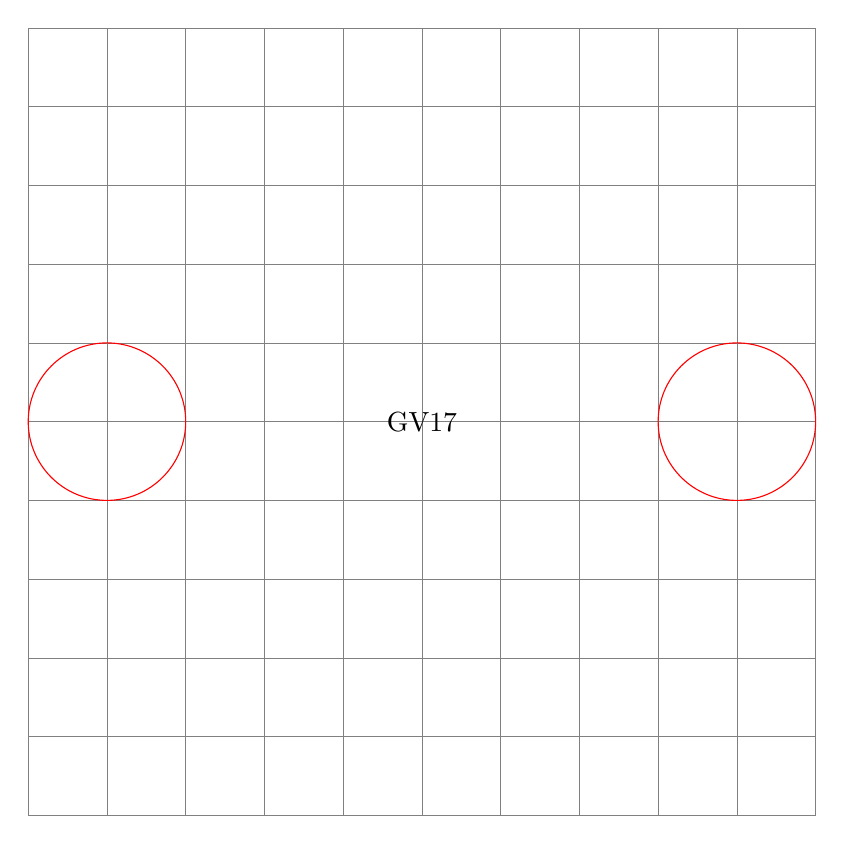
\begin{tikzpicture}
        \coordinate (GV17) at (0,0);
        \coordinate [left  = 4 of GV17] (left_nipple);
        \coordinate [right = 4 of GV17] (right_nipple);
        \draw[step=1,gray,very thin] (-5,-5) grid (5,5);
        \node at (GV17) {GV17};
        \draw [color=red] (left_nipple) circle (1);
        \draw [color=red] (right_nipple) circle (1);
    \end{tikzpicture}
\end{document}
